\newpage
\section{Auswertung}
\label{sec:Auswertung}

\subsection{Heizrate}
Zunächst ist es sinnvoll die Heizrate bei dem Versuch zu untersuchen, da diese händisch immer wieder nachgeregelt und dardurch verändert wurde. Dazu bietet sich an 
die gemessene Temperatur gegen die Zeit aufzutragen und eine lineare Regression durchzuführen.

Die gefittete Funktion hat die Form
\begin{equation*}
  T(t) = b \cdot t + T_0 \, .
\end{equation*}

\noindent
Aus dieser, dass für die Messung in 1,5er Temperaturschritten eine Heizrate $b_1$ und bei 2er Temperaturschritten eine Heizrate von $b_2$ vorliegt. 
\begin{align*}
  &b_1 = \SI{1.41(13)}{\kelvin\per\minute} \\
  &b_2 = \SI{1.93(33)}{\kelvin\per\minute} \, .
\end{align*}

Die Notation die Variablen die sich auf die Messung mit 1,5er Temperaturschritten bezieht mit $_1$ und die Variablen welche sich auf die Messung mit 2er Temperaturerhöhungsschritten 
bezieht mit $_2$ zu vermerken wird in dem gesamten \autoref{sec:Auswertung} und \autoref{sec:Diskussion} beibehalten.

\noindent
Die \autoref{fig:2-linregress} sind mit den entsprechenden gefitteten Funktion aufgetragen.

\begin{figure}
  \label{fig:2-linregress}
  \centering
  \begin{subfigure}[b]{0.45\textwidth}
      \centering
      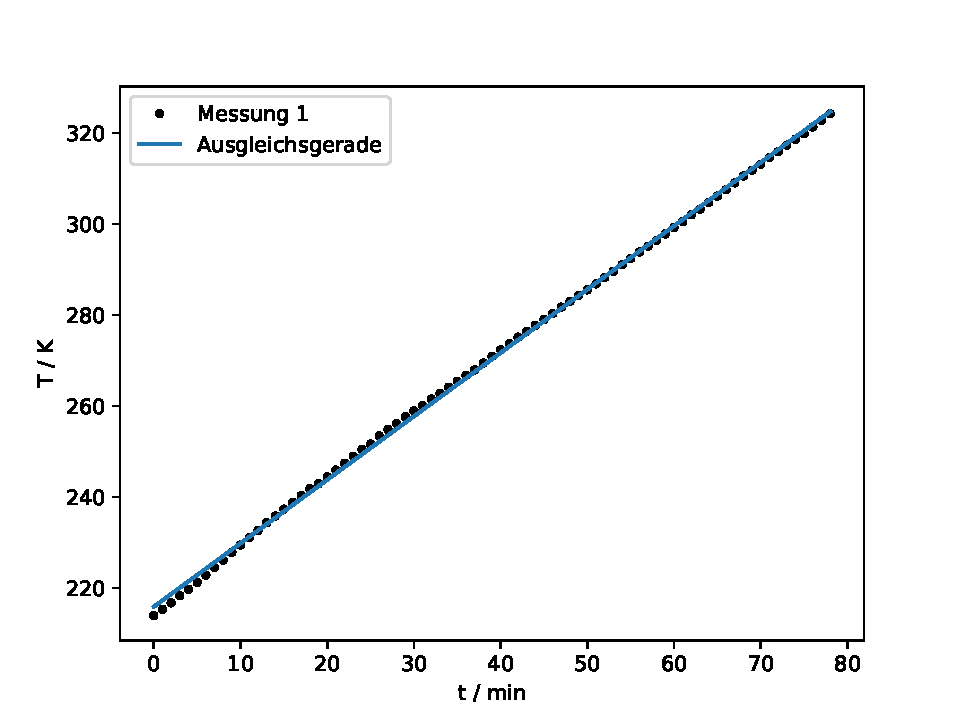
\includegraphics[width=\textwidth]{build_j/zeit_temp_fit_1.pdf}
      \caption{Die gemessene Temperatur gegen die Zeit aufgetragen für die Messung 1 inklusive Fit Funktion}
  \end{subfigure}
  \hfill
  \begin{subfigure}[b]{0.45\textwidth}
      \centering
      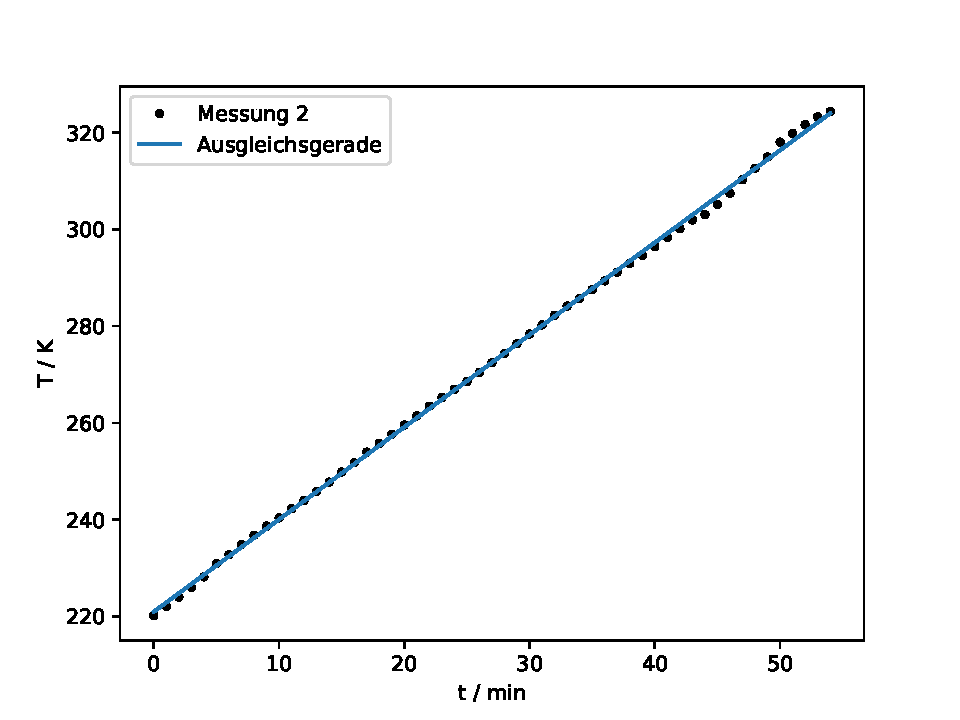
\includegraphics[width=\textwidth]{build_j/zeit_temp_fit_2.pdf}
      \caption{Die gemessene Temperatur gegen die Zeit aufgetragen für die Messung 2 inklusive Fit Funktion}
  \end{subfigure}
  \caption{}
\end{figure}


\subsection{Untergrund}

Da bei der Messung der Daten nicht nur der Strom der durch die Dipolrelaxationen im Kristall gemessen wurde, sondern auch ein exponentiell wachsender Untergrund, ist es sinnvoll
für die weitere Auswertung diese durch eine e-Funktion der Form 
\begin{equation*}
  f(T) = a \cdot \exp(-\frac{m}{T})
\end{equation*}

\noindent 
zu approximieren. Das Temperatur-Strom Diagramm inklusive der gefitteten e-Funktion ist in \autoref{fig:Untergrund} zu sehen. Der Fit wird versucht an das 2. Maxima zu legen. 
Daraus folgen folgende Werte:

\begin{align*}
  &\text{Messung 1}\\
  &a =  \SI{6.197(3794)e11}{\pico\ampere} &&  m = \SI{7282.75(18414)}{\kelvin} \, ,\\
  &\text{Messung 2}\\
  &a = \SI{1.263(617)e11}{\pico\ampere} &&  m = \SI{6729.57(15056)}{\kelvin} \, .\\ 
\end{align*}


\begin{figure}
  \label{fig:Untergrund}
  \centering
  \begin{subfigure}[b]{0.75\textwidth}
      \centering
      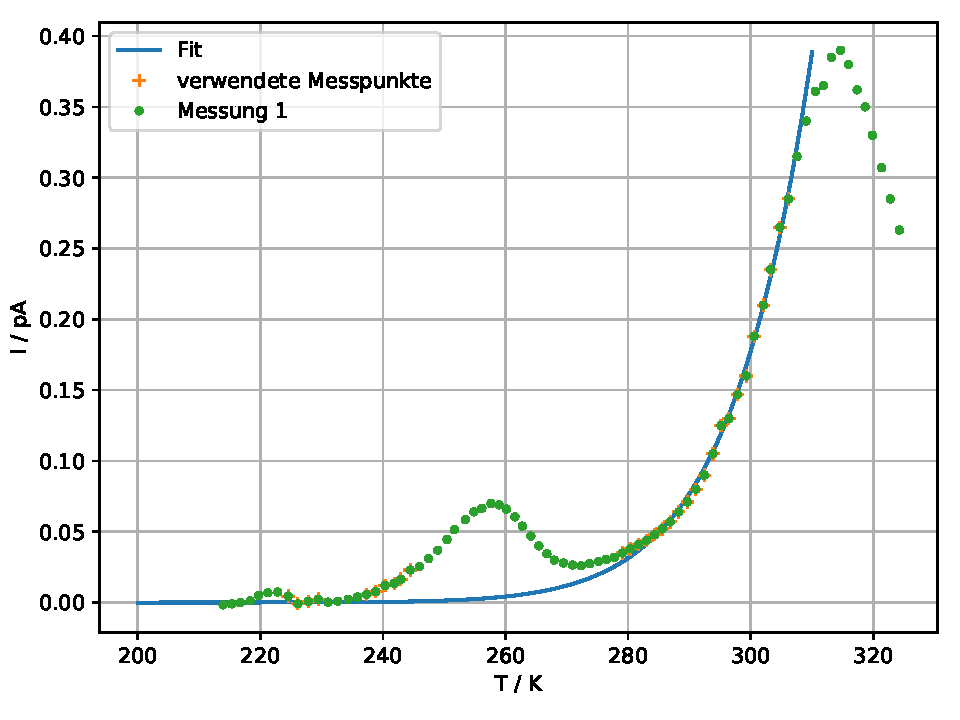
\includegraphics[width=\textwidth]{build_j/untergrund_1.pdf}
      \caption{Die gemessene Temperatur gegen den gemessenen Strom aufgetragen für die Messung 1 inklusive Fit für den Untergrund}
  \end{subfigure}
  \hfill
  \begin{subfigure}[b]{0.75\textwidth}
      \centering
      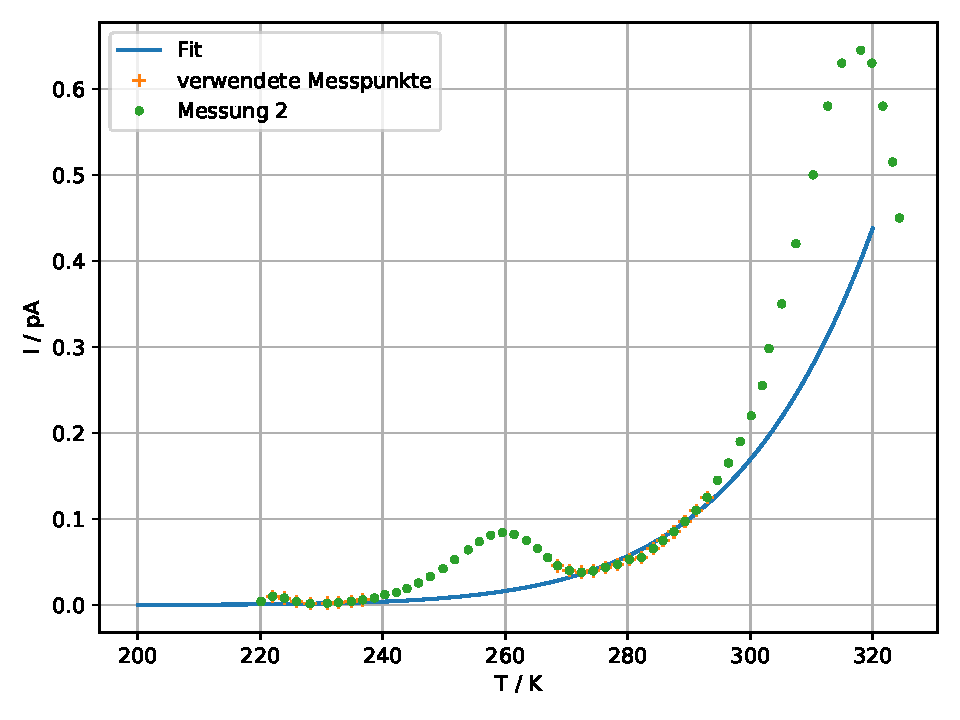
\includegraphics[width=\textwidth]{build_j/untergrund_2.pdf}
      \caption{Die gemessene Temperatur gegen den gemessenen Strom aufgetragen für die Messung 1 inklusive Fit für den Untergrund}
  \end{subfigure}
  \caption{}
\end{figure}

\subsection{Berechnung der Aktivierungsenergie über den Strom}


